\documentclass[12pt]{article}
\usepackage[a4paper, total={6in, 9in}]{geometry}
\usepackage{graphicx}
\graphicspath{ {./images/output/} }
\usepackage{caption}
\usepackage[english]{babel}
\usepackage{titling}
\usepackage{float}
% \usepackage{amsmath}
% \usepackage{minted}
% \usepackage{multicol}
% \usepackage{array}
% \usepackage{setspace}
% \usepackage{placeins}

% \usepackage{lipsum}

\title{Study of 3-\(\Phi\) Star Rectifier using Diode, \& Thyristor with R, RL Load}
\author{}
\date{}

\pagenumbering{gobble}
\begin{document}
\vspace*{\fill}
\begin{center}

    \emph{Heaven's Light is Our Guide} \\
    \textbf{Rajshahi University of Engineering and Technology} \\

    \begin{figure}[H]
        \centering
        
\includegraphics[scale=.34]{images/RUET_logo.png}
        \label{fig:ruet_logo}
    \end{figure}
    \vspace{5mm}

    \textbf{Course Code}\\
    ECE 3206\\
    \vspace{3mm}
    \textbf{Course Title}\\
    Industrial Electronics Sessional

    \vspace{5mm}
    \textbf{Experiment Date:} {January 13, 2025},\\
    \textbf{Submission Date:} {February 10, 2025}\\

    \vspace{5mm}
    \textbf{Lab Report 3: \\
        Study of Thyristor Characteristics R, RL Load}

    \vspace{15mm}

    \begin{tabular}{c|c}
        \textbf{Submitted to} & \textbf{Submitted by} \\
        Md. Faysal Ahamed     & Md. Tajim An Noor     \\
        Lecturer              & Roll: 2010025         \\
        Dept of ECE, Ruet     &                       \\
    \end{tabular}

\end{center}
\vspace*{\fill}


\pagebreak

\tableofcontents

\pagebreak
\pagenumbering{arabic}
\maketitle

\section*{Theory}
\addcontentsline{toc}{section}{Theory}
A three-phase star rectifier is a type of rectifier circuit that converts three-phase AC (Alternating Current) input into DC (Direct Current) output. This type of rectifier is commonly used in industrial applications due to its efficiency and ability to handle high power levels \cite{power_electronics}.
\\\\
In a three-phase star rectifier, diodes are arranged in a star configuration. Each phase of the AC supply is connected to a diode, and the other ends of the diodes are connected together to form the DC output. The rectifier can be used with different types of loads, such as resistive (R) and inductive-resistive (RL) loads \cite{rectifier_design}.
\\\\
When a resistive load is used, the current through the load is in phase with the voltage, resulting in a purely resistive circuit. However, when an inductive-resistive load is used, the current lags behind the voltage due to the inductance, creating a more complex circuit behavior \cite{electrical_machines}.
\\\\
Thyristors, also known as silicon-controlled rectifiers (SCRs), can be used in place of diodes in a three-phase star rectifier to provide controlled rectification. By adjusting the gate signal of the thyristors, the conduction angle can be controlled, allowing for regulation of the output voltage. This makes thyristors suitable for applications where variable DC output is required \cite{thyristor_control}.
\\\\
When using thyristors with a resistive load, the output voltage can be controlled by varying the gate signal, which delays the conduction angle and reduces the average output voltage. For an inductive-resistive load, the current lags behind the voltage, and the gate signal delay further affects the conduction angle and the current waveform \cite{power_electronics}.
\\\\
MATLAB/Simulink is a powerful tool for simulating and analyzing the performance of such rectifier circuits. By using MATLAB/Simulink, we can model the three-phase star rectifier with both diodes and thyristors and observe the output waveforms for different load conditions. This helps in understanding the behavior of the rectifier and optimizing its performance for various industrial applications \cite{simulink_guide}.


\section*{Required Equipments/Software}
\addcontentsline{toc}{section}{Required Equipments/Software}
\begin{itemize}
    \item MATLAB/Simulink
    \item Oscilloscope
    \item AC Voltage Source
    \item Diode
    \item Thyristor
    \item Series RLC Branch
    \item Pulse Generator
    \item Measurement Tools
\end{itemize}

\section*{Circuit Diagrams}
\addcontentsline{toc}{section}{Circuit Diagrams}
\begin{figure}[H]
    \centering
    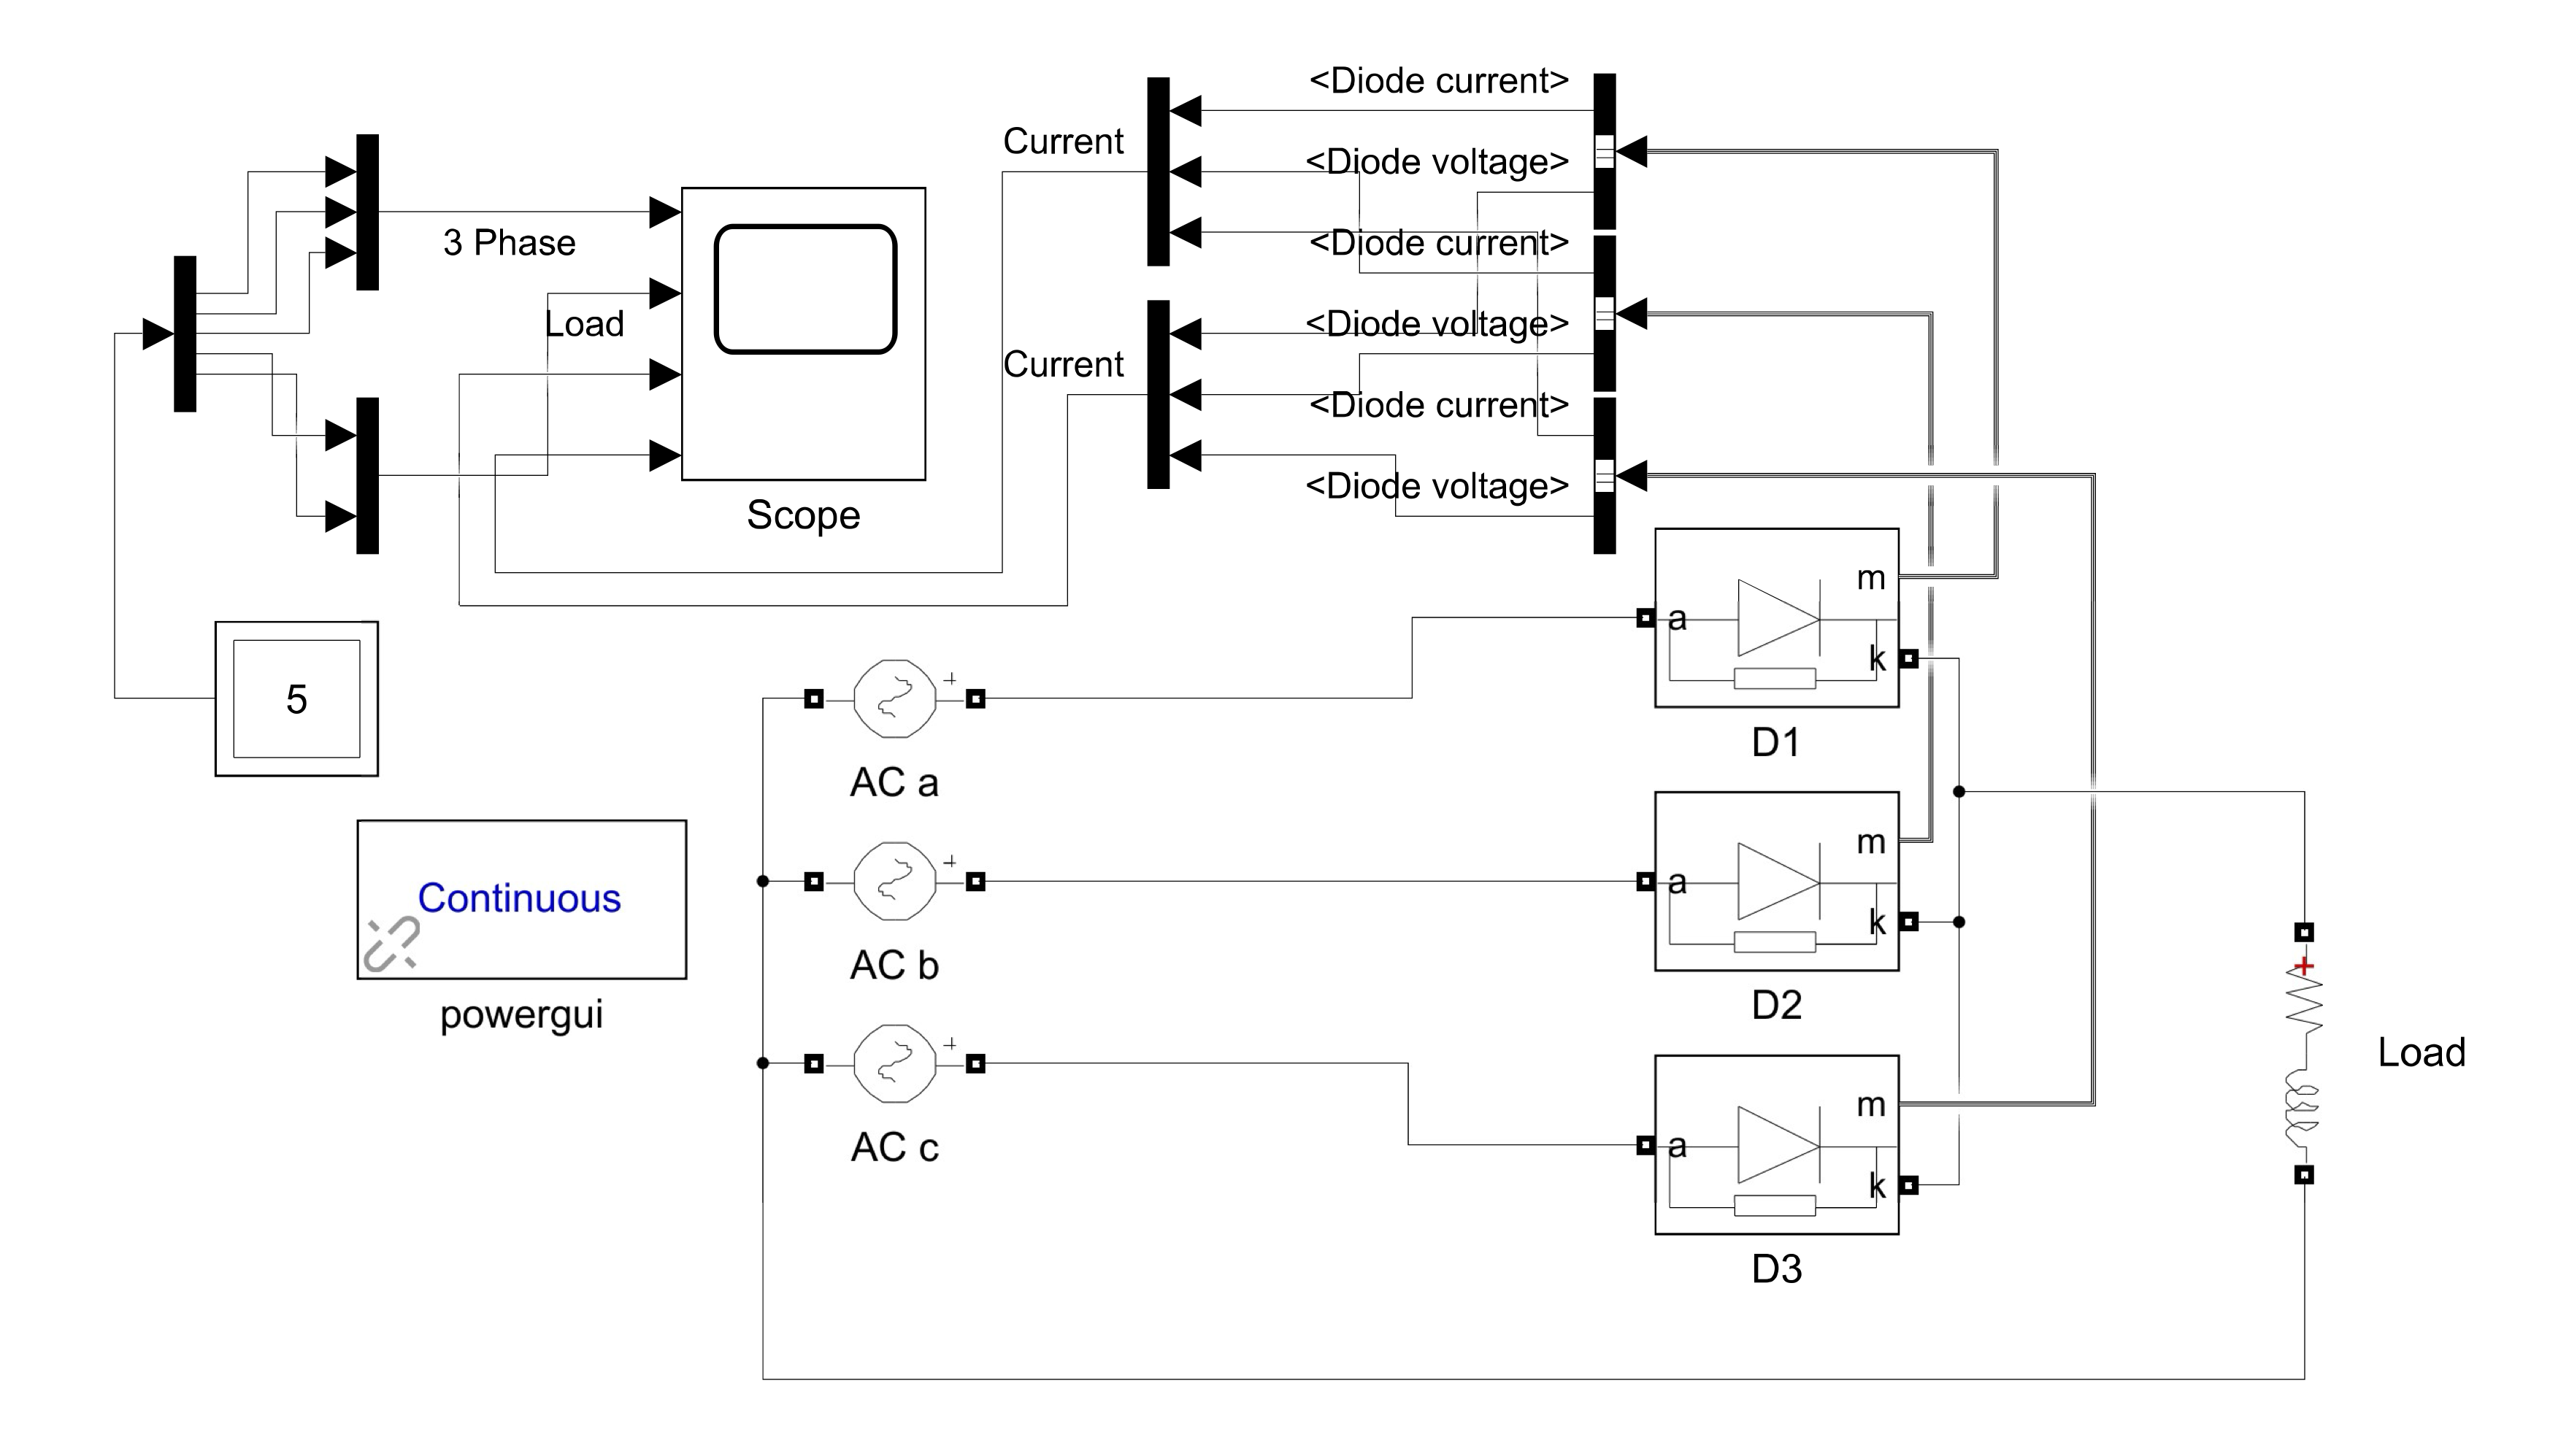
\includegraphics[width=\textwidth]{ckt.png}
    \caption{3-Phase Star Rectifier with Diode}
    \label{fig:d_load}
\end{figure}

\begin{figure}[H]
    \centering
    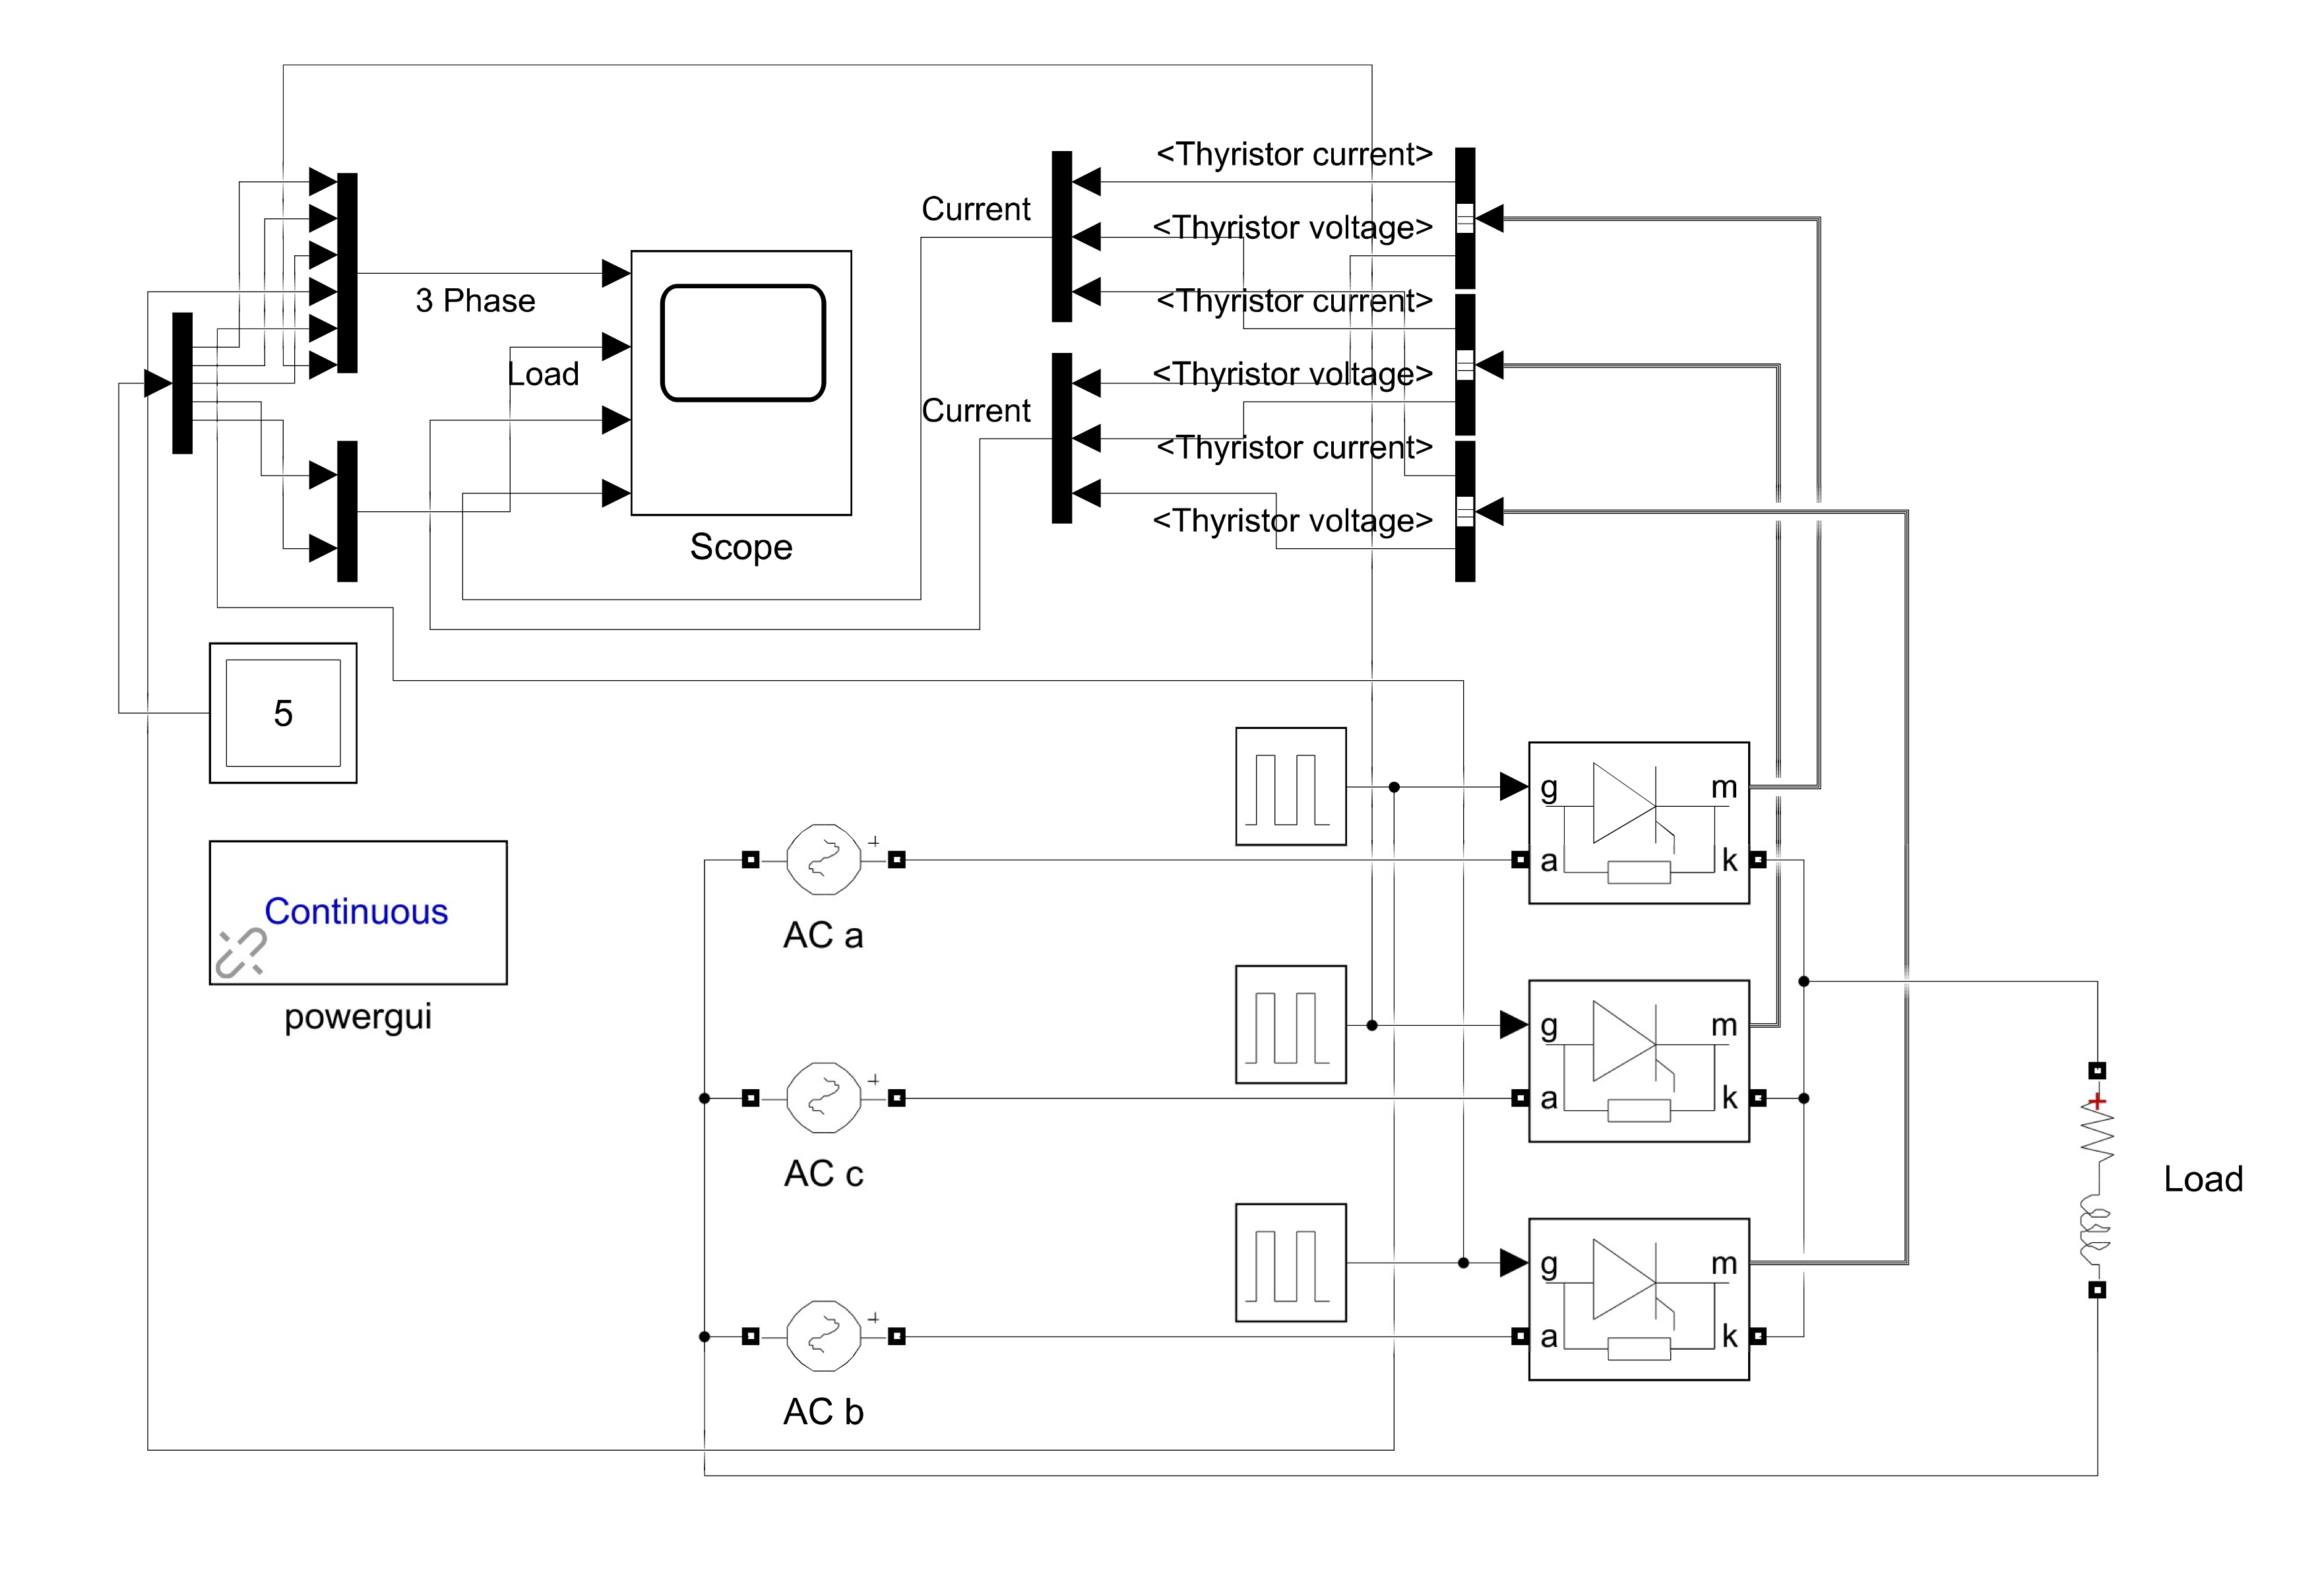
\includegraphics[width=\textwidth]{ckt2.png}
    \caption{3-Phase Star Rectifier with Thyristor}
    \label{fig:t_load}
\end{figure}

\section*{Observations}
\addcontentsline{toc}{section}{Observations}
\begin{itemize}
    \item The output voltage for the R load is a pulsating DC with a frequency 6 times the input AC.
    \item With gate voltage delay for the thyristor and R load, the output voltage shows a delayed conduction angle, reducing the average output.
    \item For the RL load, the output voltage is pulsating DC, with the current lagging due to inductance.
    \item Gate voltage delay for the thyristor with RL load results in a delayed conduction angle and a more pronounced current lag.
    \item Thyristor with 15-degree gate delay and R load: reduced average output due to delayed conduction.
    \item Thyristor with no gate delay and R load: output similar to diode rectifier with controlled conduction.
    \item Thyristor with 15-degree gate delay and RL load: delayed conduction and increased current lag.
    \item Thyristor with no gate delay and RL load: output similar to diode rectifier with controlled conduction.
    \item MATLAB/Simulink helps analyze and visualize rectifier performance.
\end{itemize}


\subsubsection*{Outputs}
\begin{figure}[H]
    \centering
    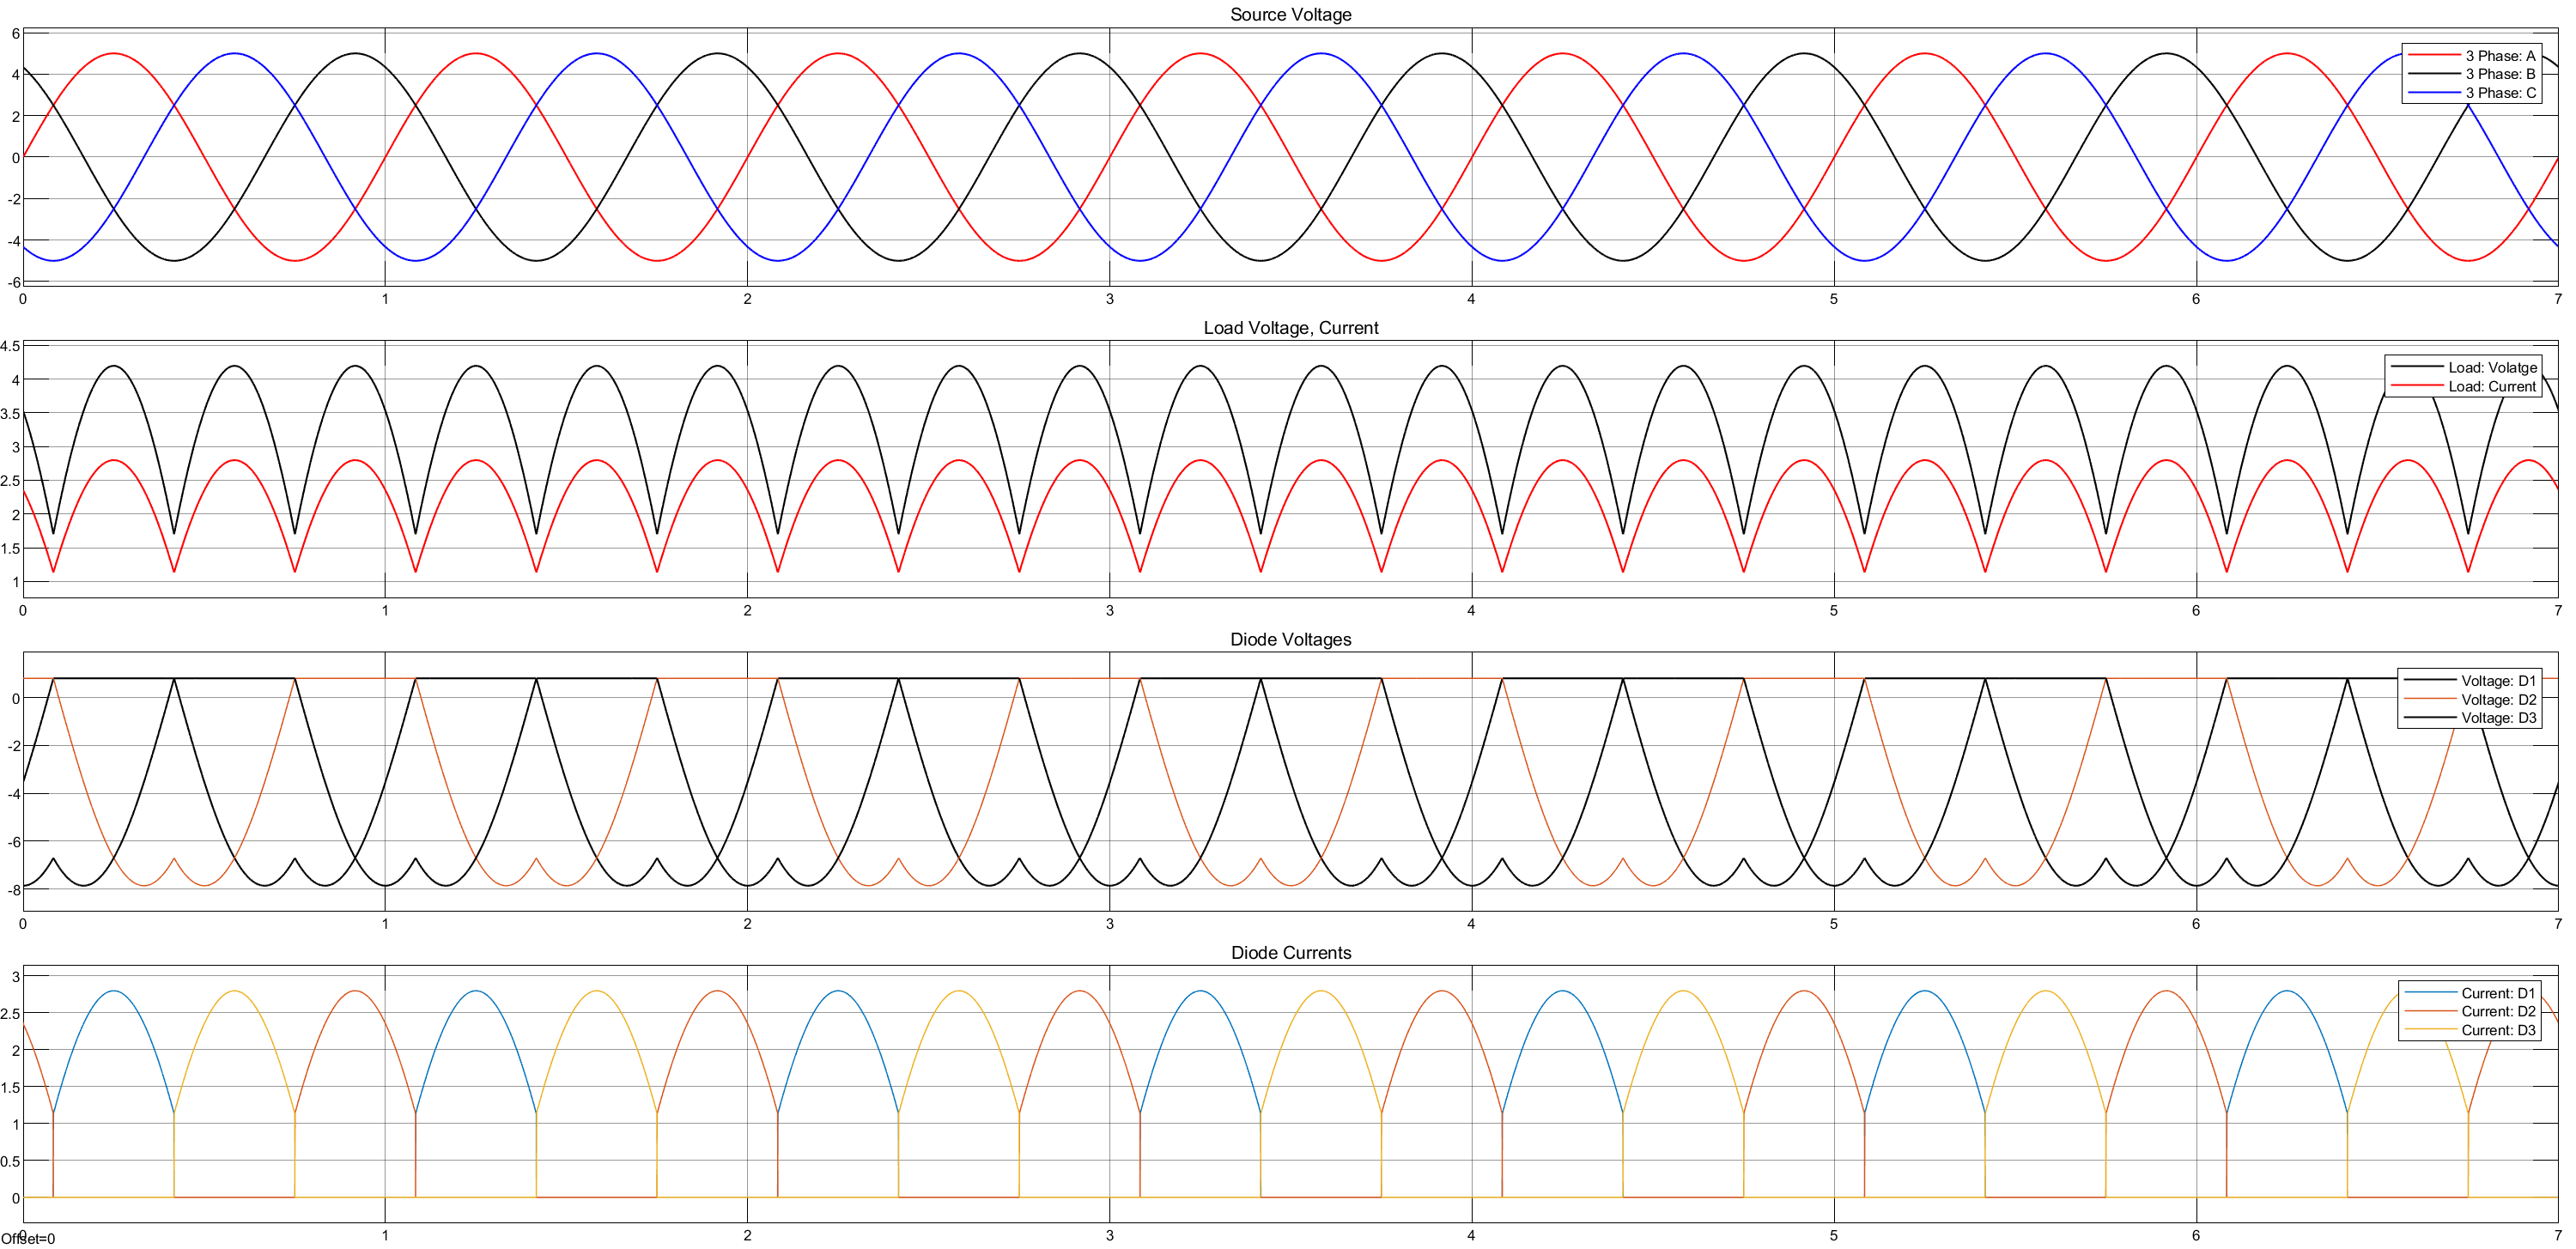
\includegraphics[width=\textwidth]{r.png}
    \caption{Simulation Output for R Load, 3-Phase Star Rectifier}
    \label{fig:rLoad}
\end{figure}

\begin{figure}[H]
    \centering
    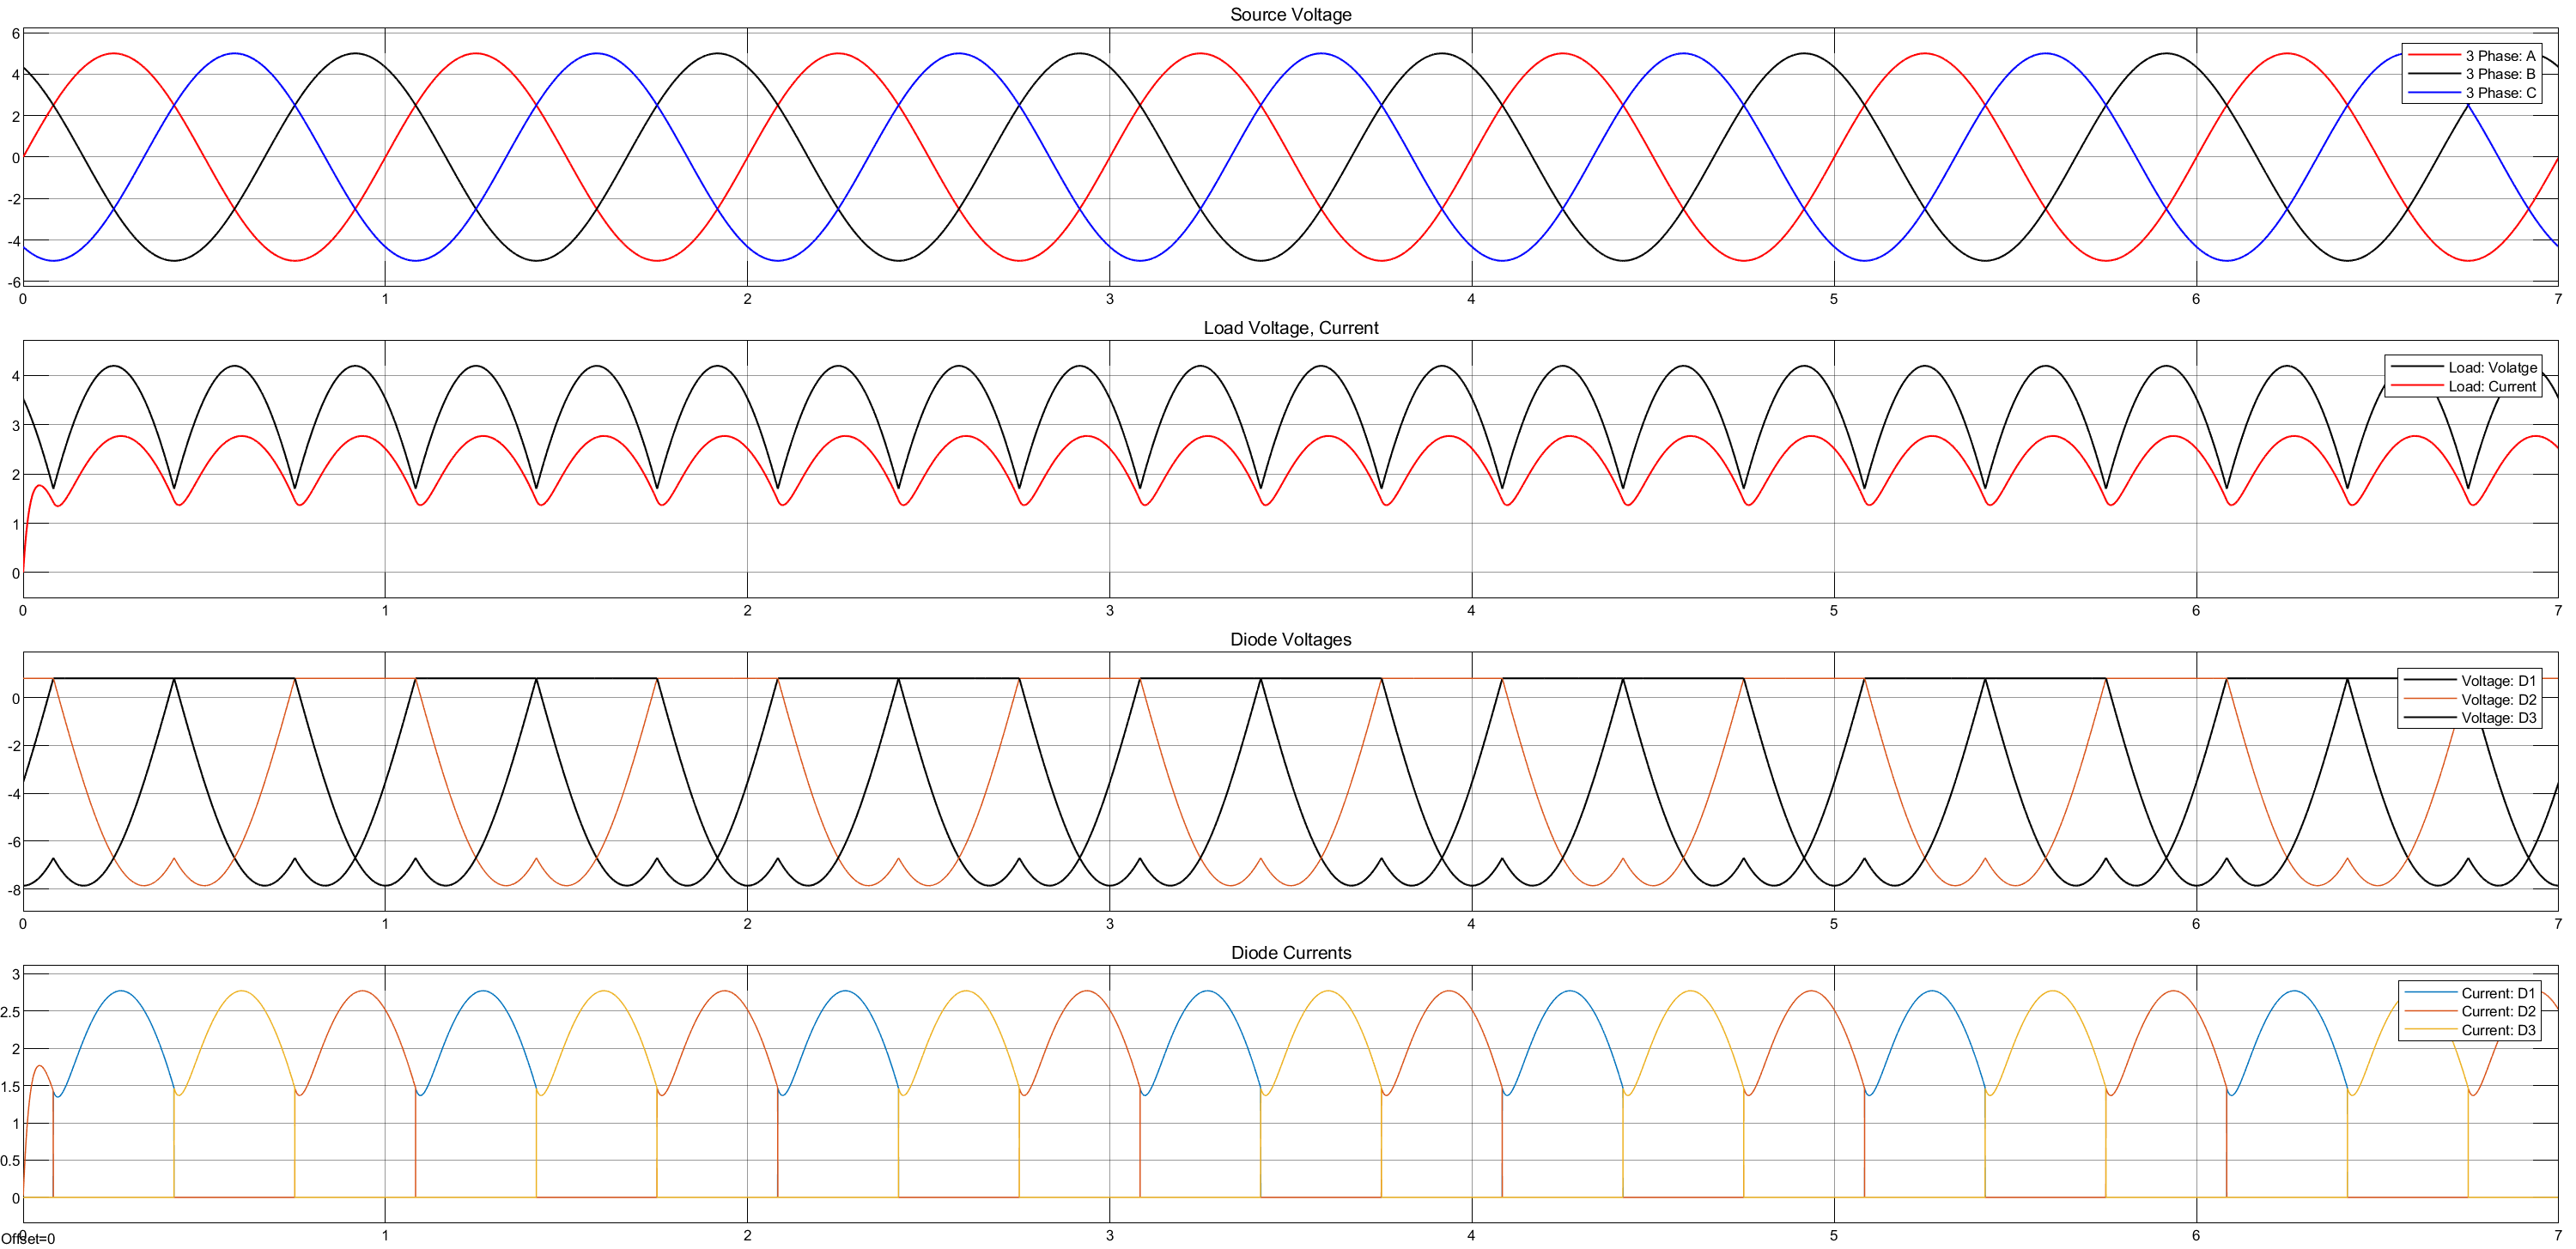
\includegraphics[width=\textwidth]{rl.png}
    \caption{Simulation Output for RL Load, 3-Phase Star Rectifier}
    \label{fig:rlLoad}
\end{figure}

\begin{figure}[H]
    \centering
    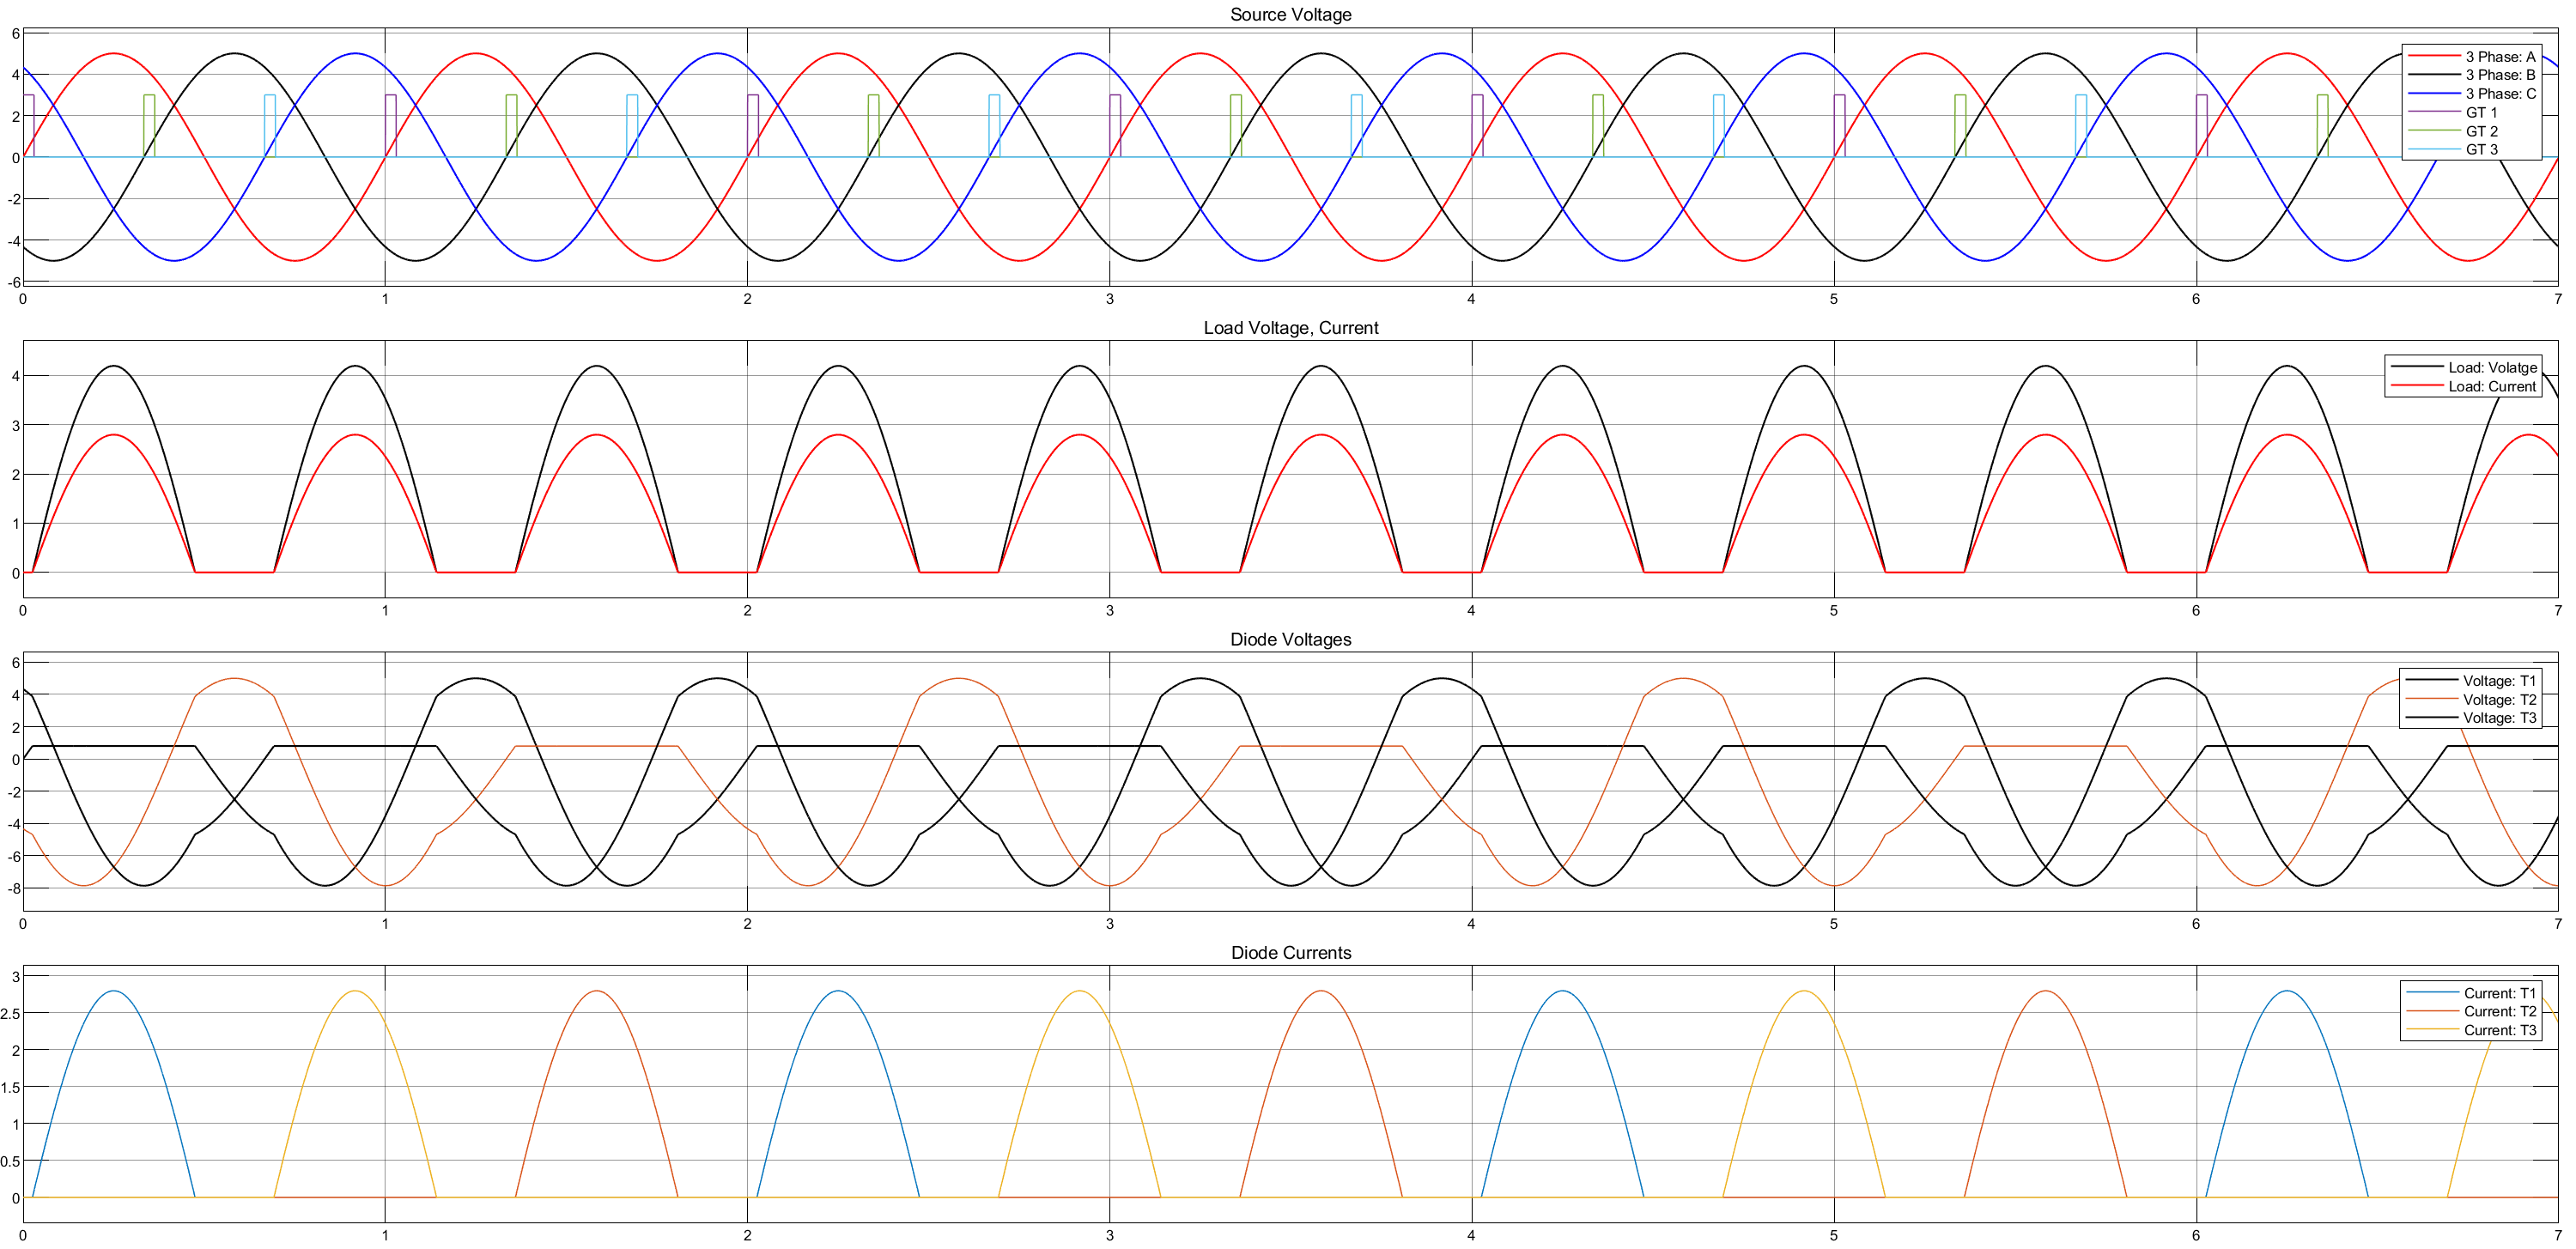
\includegraphics[width=\textwidth]{r-nd.png}
    \caption{Simulation Output for R Load, Controlled Rectifier, No Delay}
    \label{fig:rControlledNoDelay}
\end{figure}

\begin{figure}[H]
    \centering
    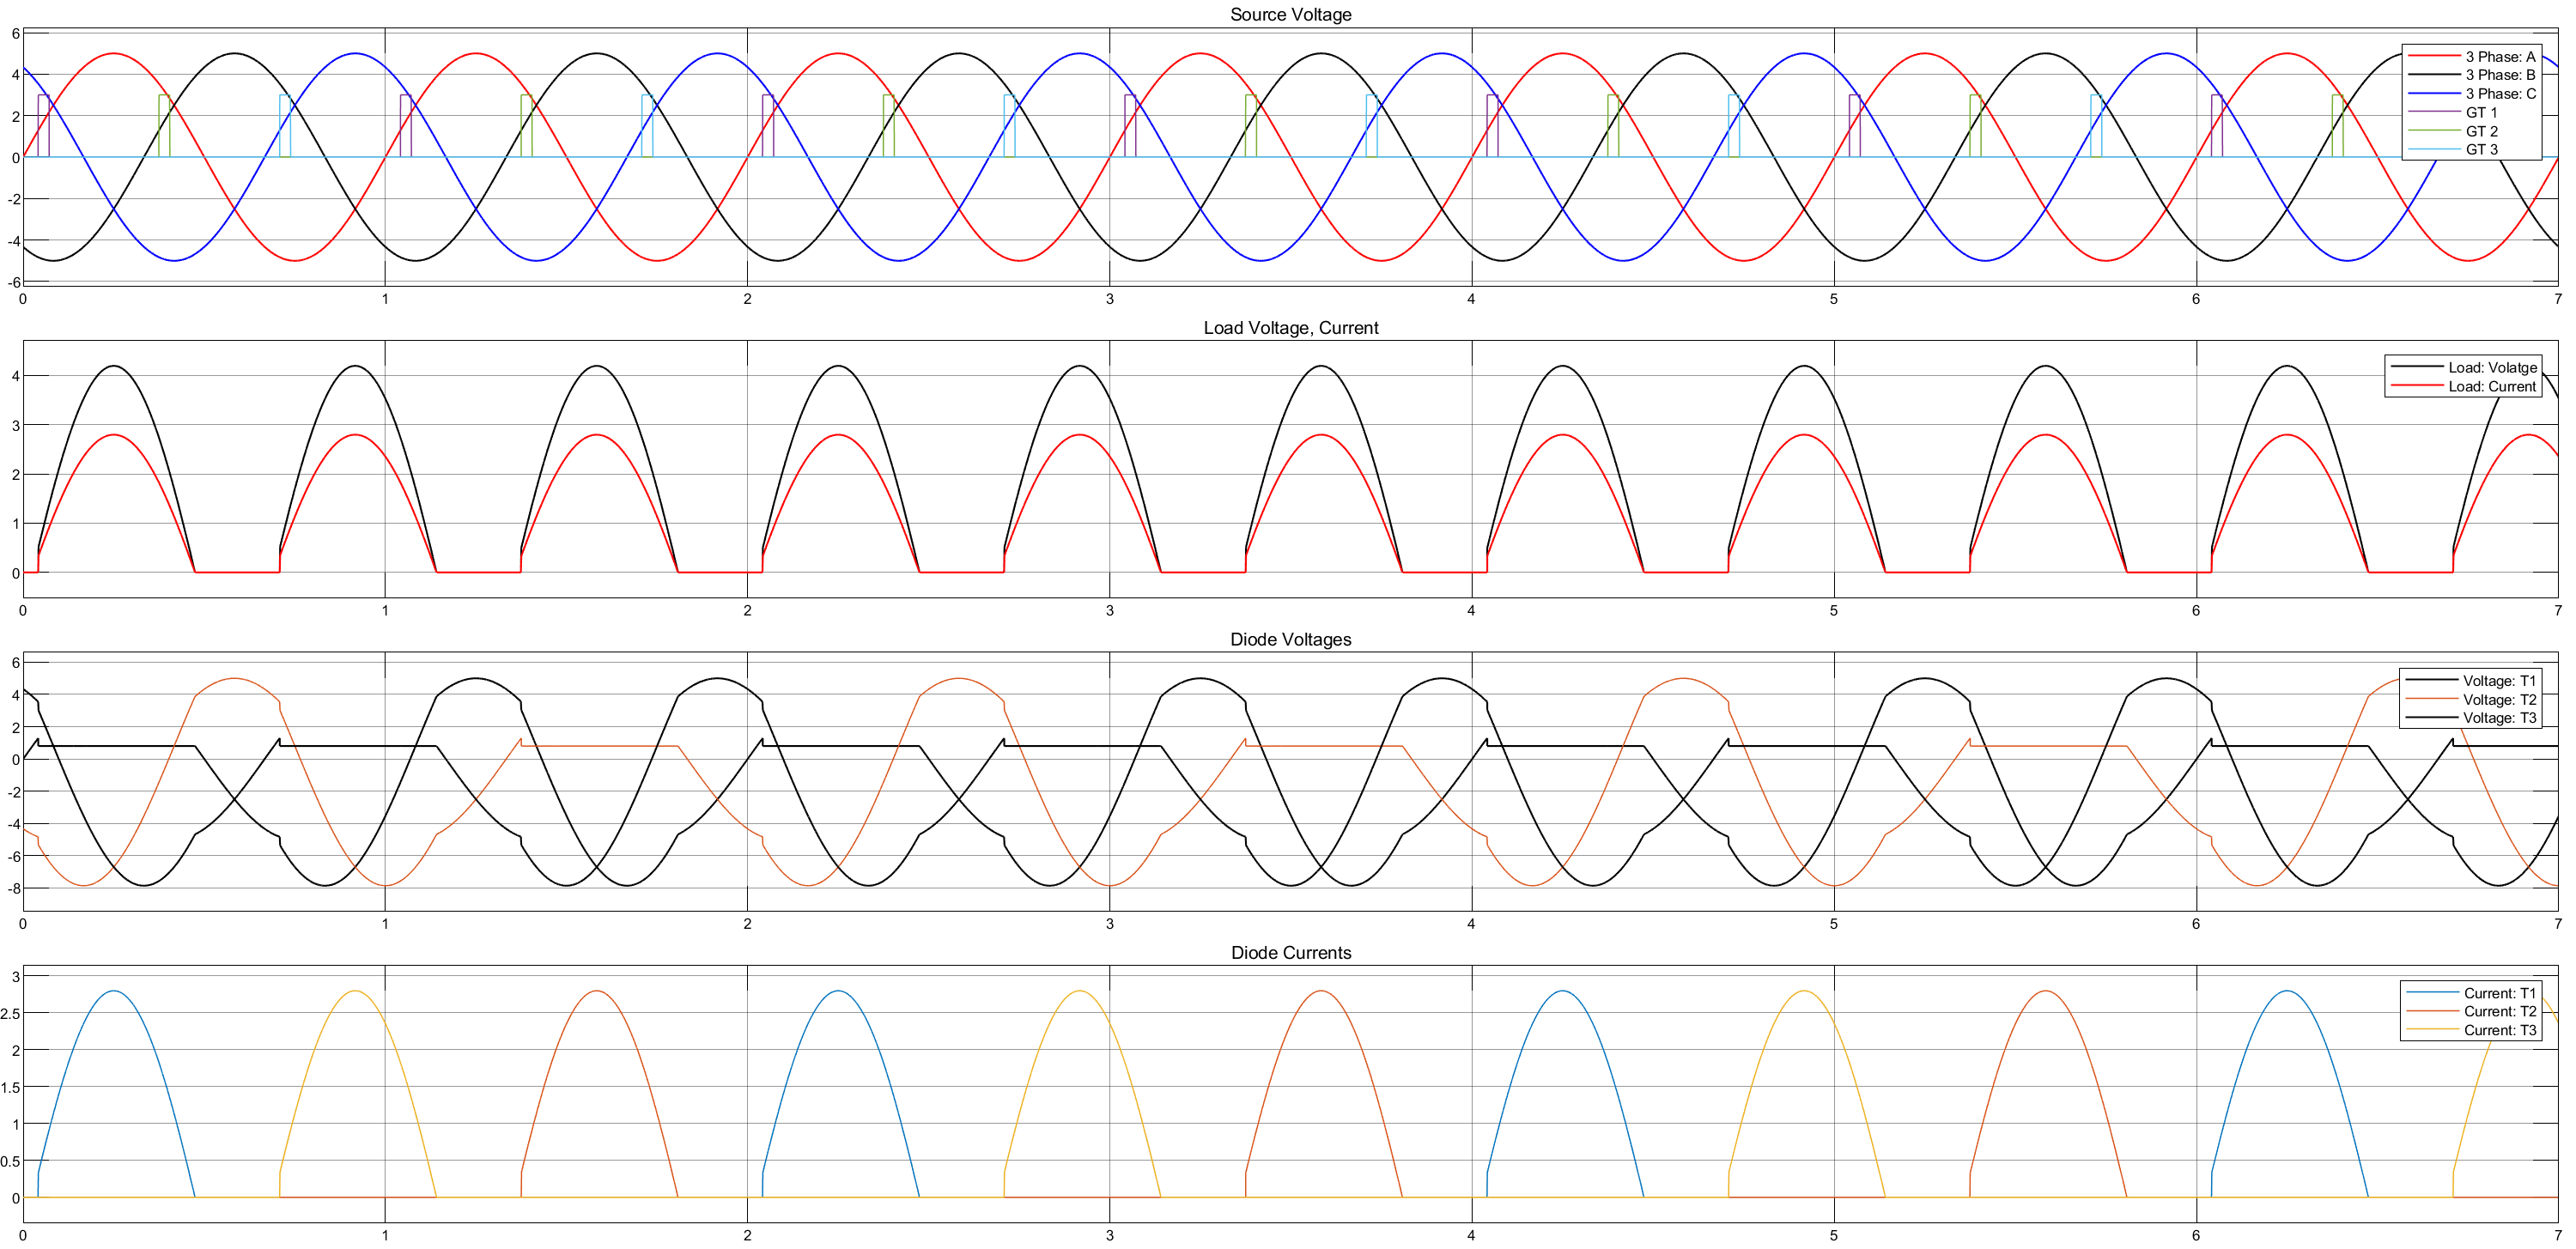
\includegraphics[width=\textwidth]{r-d.png}
    \caption{Simulation Output for R Load, Controlled Rectifier, With Delay}
    \label{fig:rControlledWithDelay}
\end{figure}

\begin{figure}[H]
    \centering
    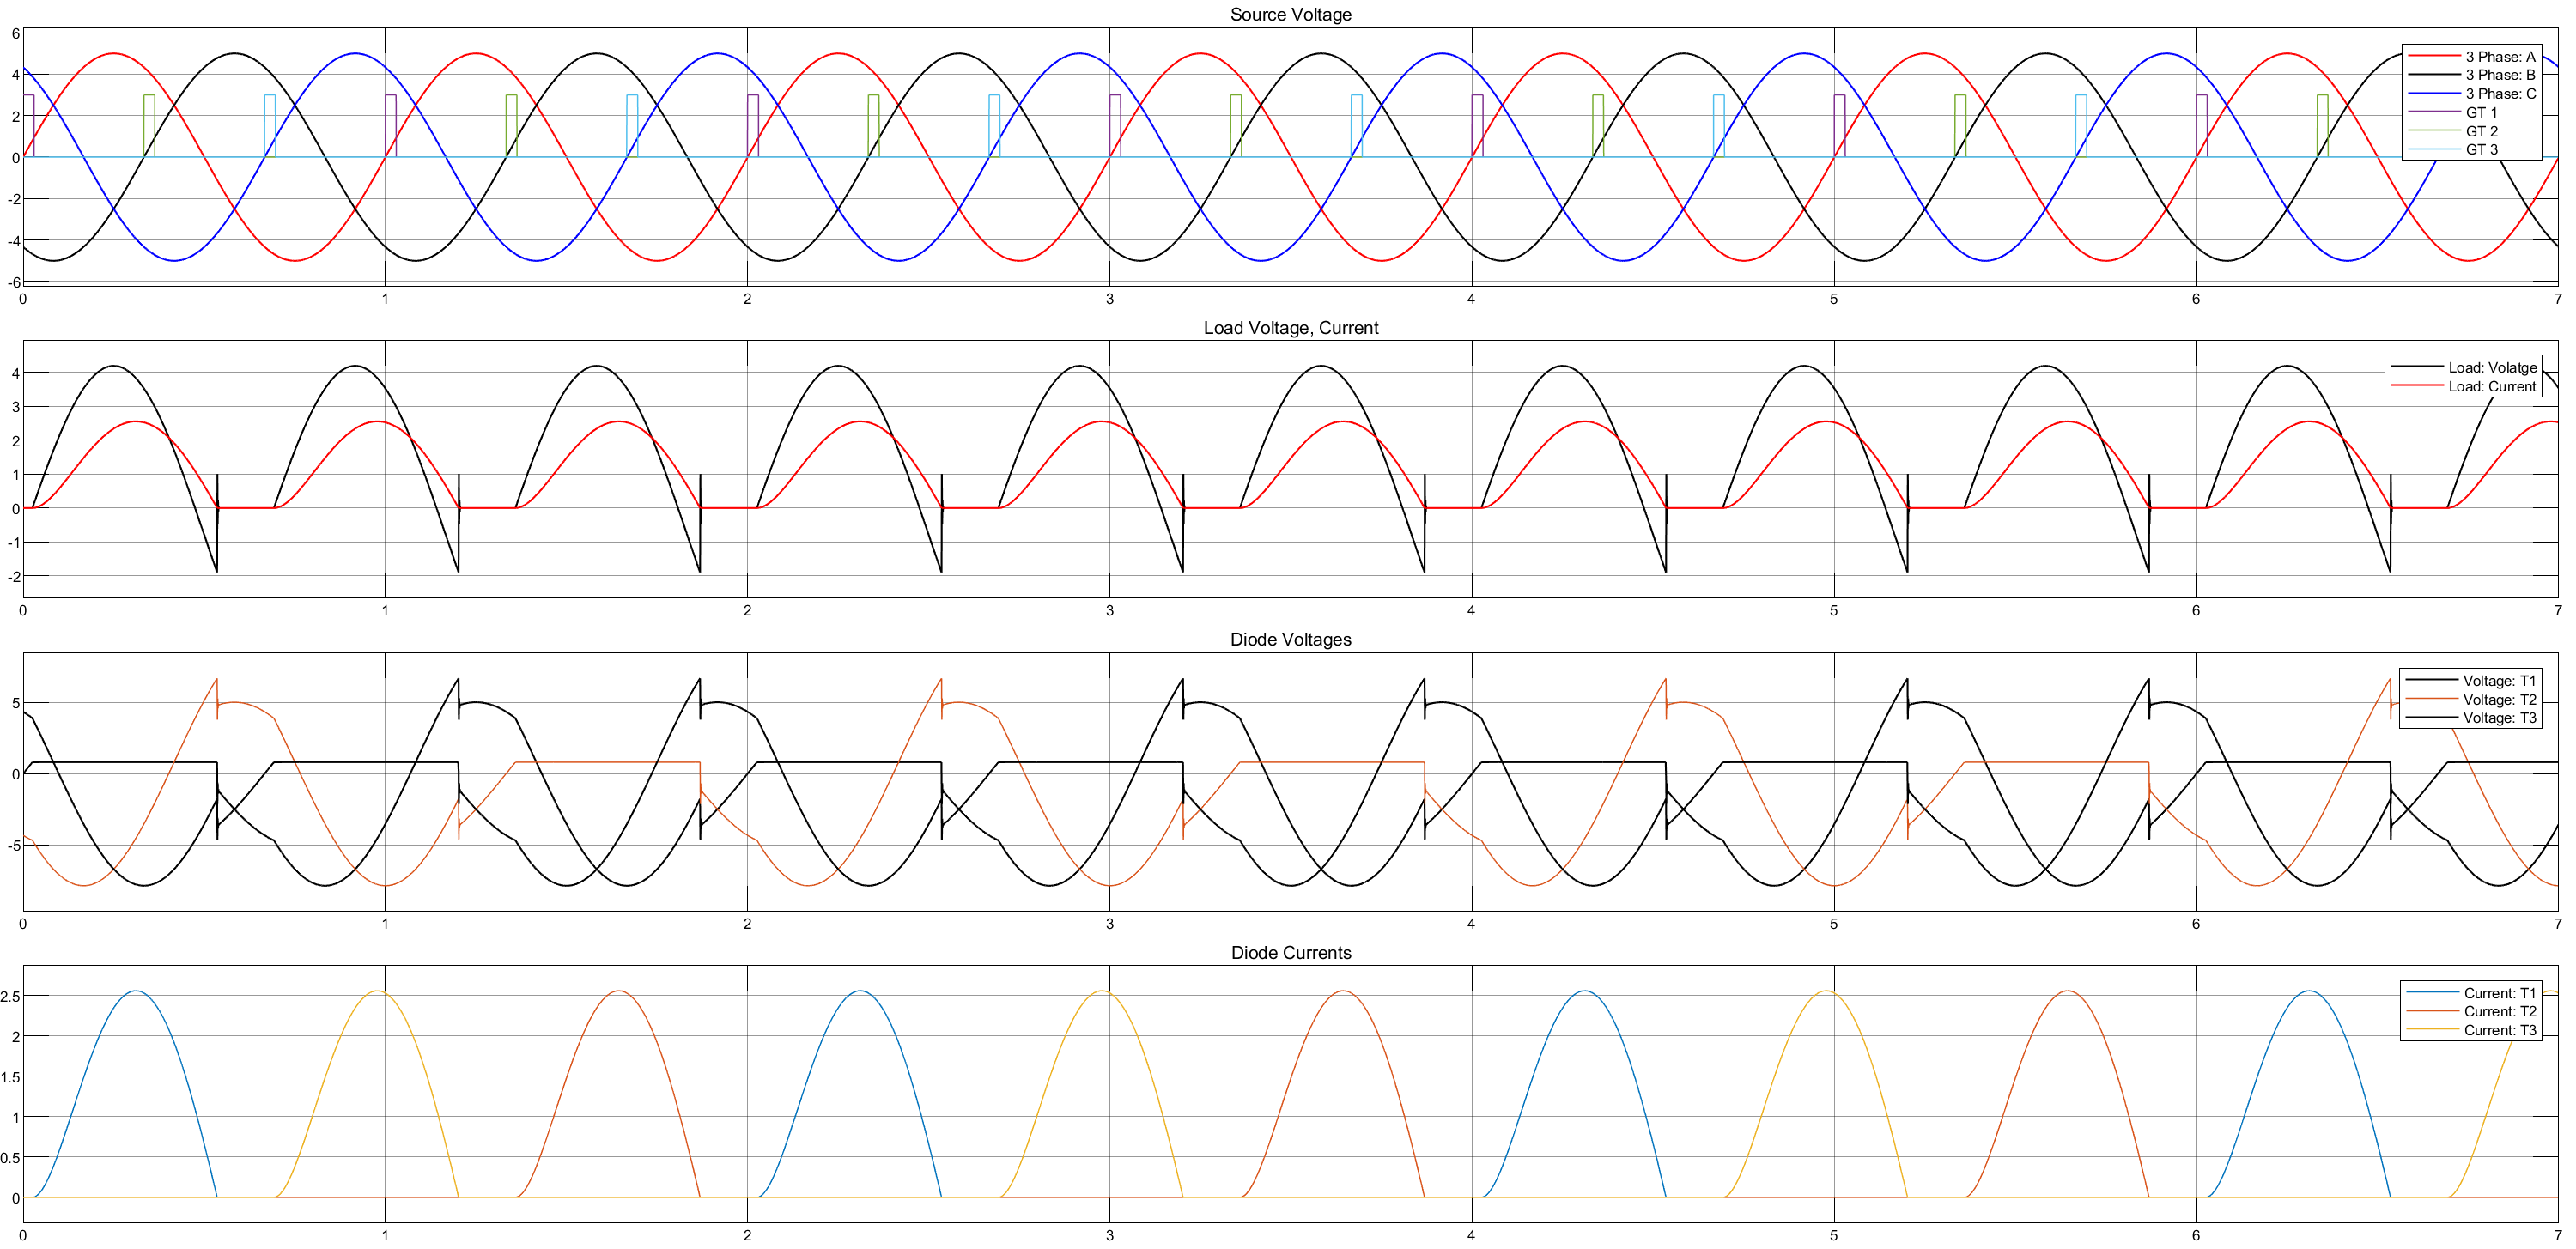
\includegraphics[width=\textwidth]{rl-nd.png}
    \caption{Simulation Output for RL Load, Controlled Rectifier, No Delay}
    \label{fig:rlControlledNoDelay}
\end{figure}

\begin{figure}[H]
    \centering
    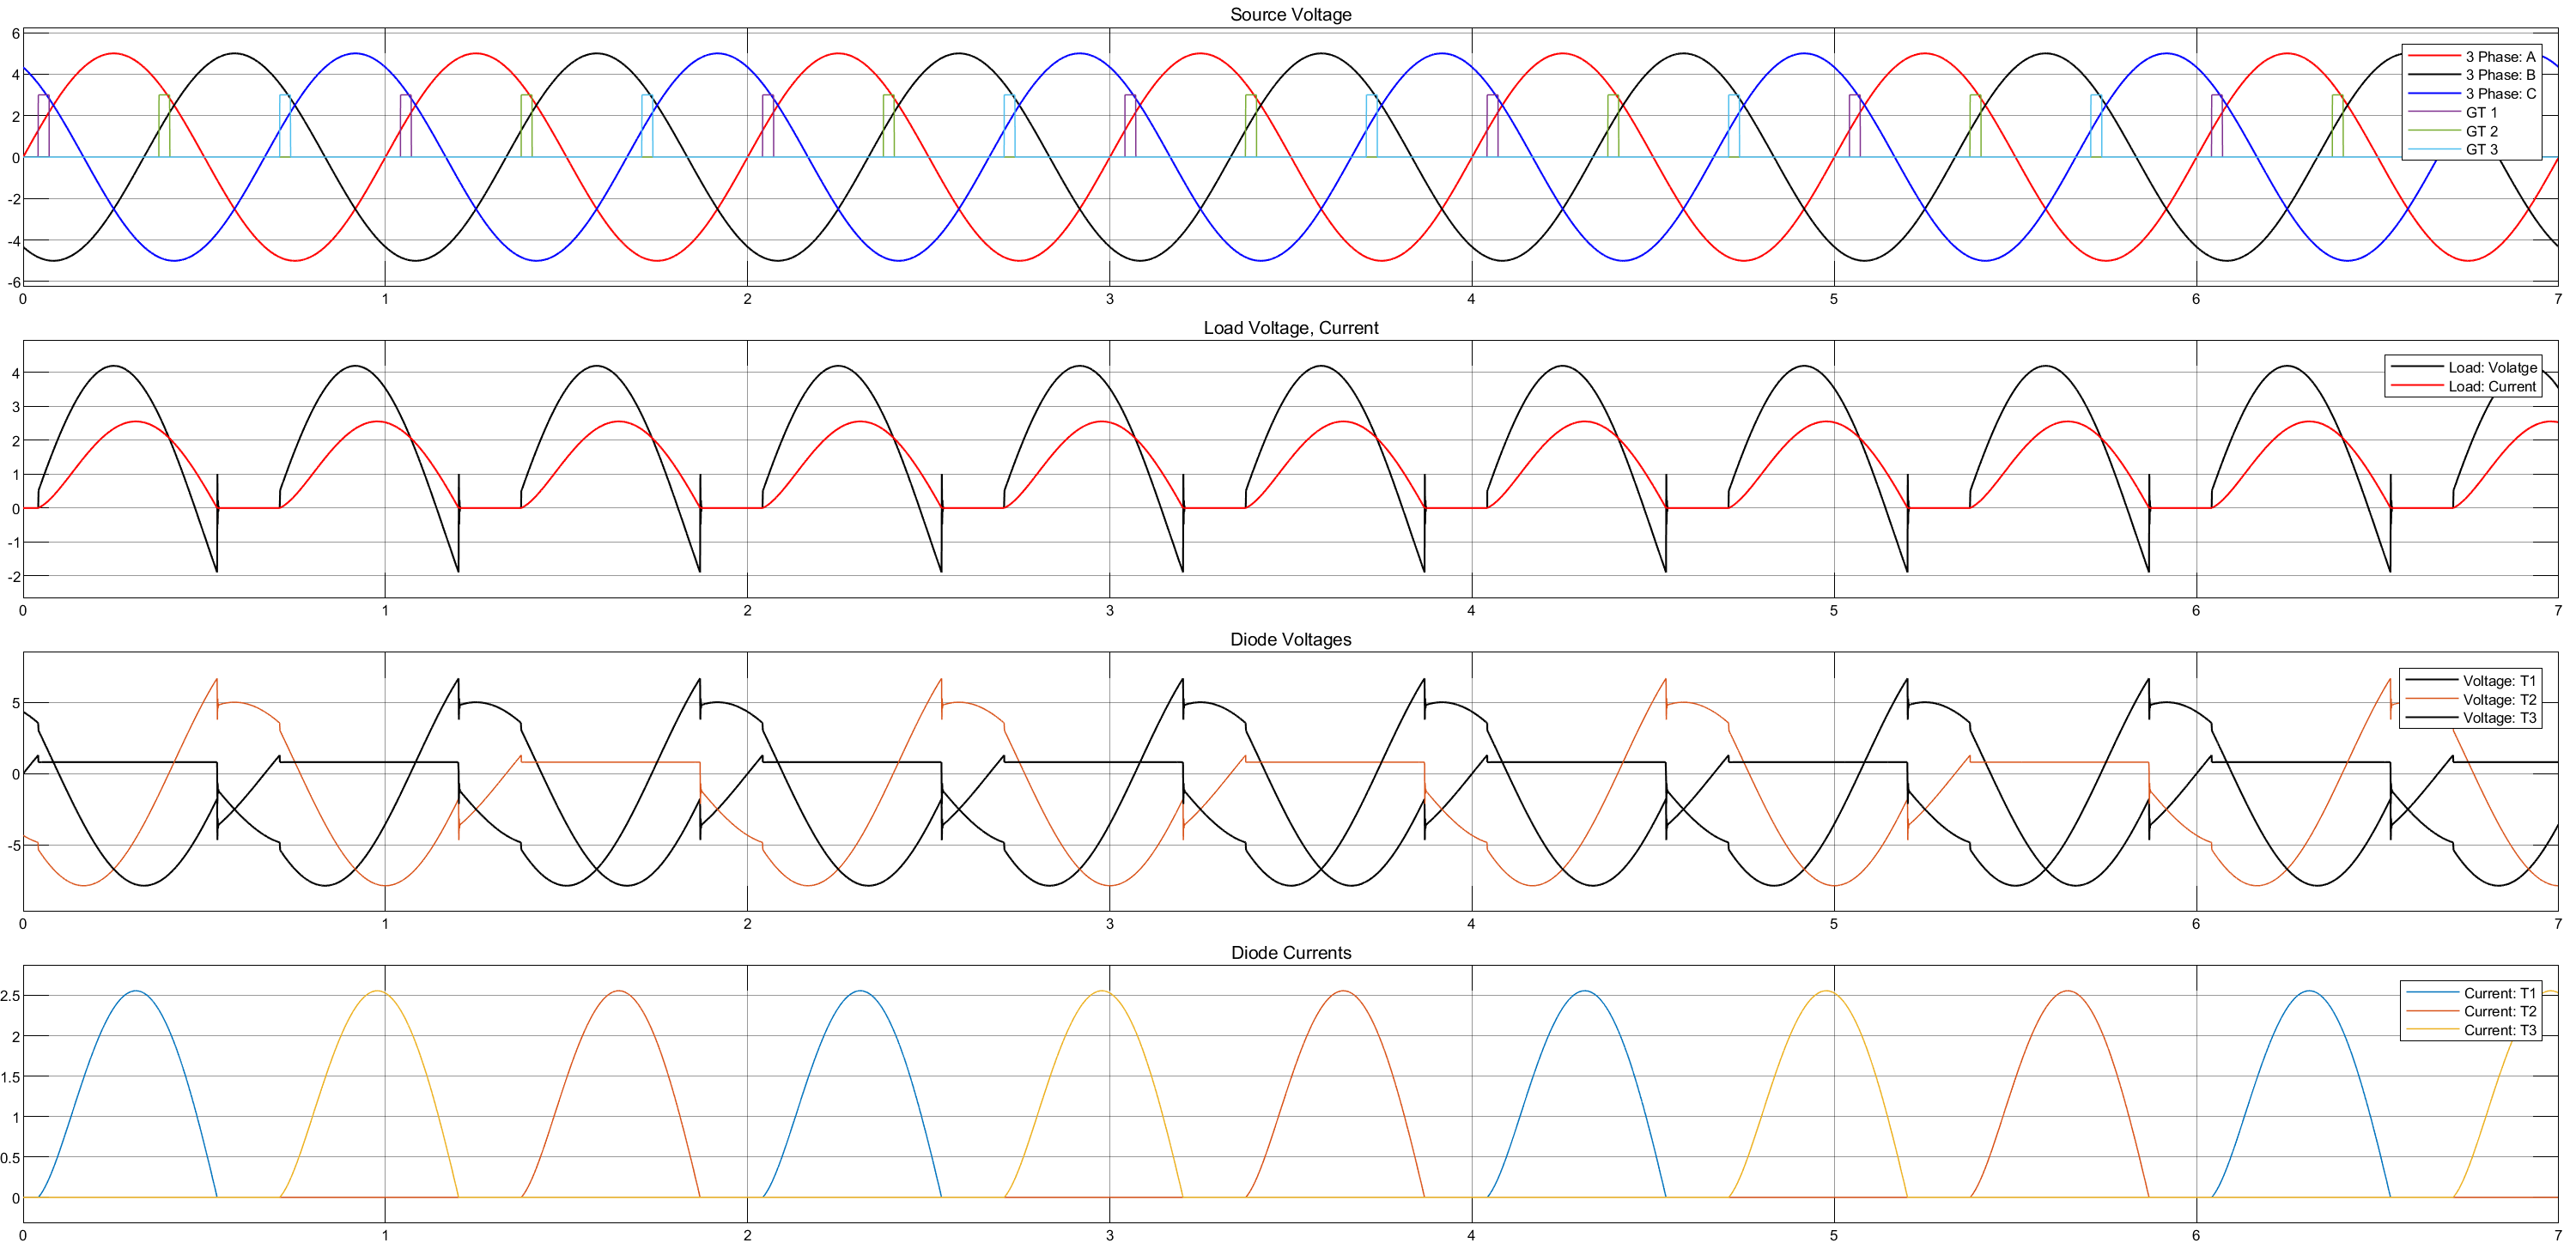
\includegraphics[width=\textwidth]{rl-d.png}
    \caption{Simulation Output for RL Load, Controlled Rectifier, With Delay}
    \label{fig:rlControlledWithDelay}
\end{figure}

\section*{Discussion}
\addcontentsline{toc}{section}{Discussion}
The three-phase star rectifier is a versatile circuit that can be used with different types of loads to convert AC input into DC output. By using MATLAB/Simulink, we can model the rectifier and analyze its performance under various conditions. The output voltage and current waveforms can be observed to understand the rectifier's behavior and optimize its performance for different industrial applications.

\section*{Conclusion}
\addcontentsline{toc}{section}{Conclusion}
The study of the three-phase star rectifier using diodes and thyristors with R and RL loads provides valuable insights into the rectifier's behavior under different load conditions. By analyzing the output waveforms using MATLAB/Simulink, we can optimize the rectifier's performance and ensure efficient power conversion in industrial applications.

\bibliographystyle{IEEEtran}
\renewcommand{\bibname}{References}
\addcontentsline{toc}{section}{References}
\bibliography{ref}

\end{document}
